\chapter{Preliminaries}
\label{chapter:preliminaries}

The following Sections describe all the concepts required for the reader to
understand the proposed method in this thesis. However, it is still assumed that
the reader has some basic knowledge about programming and computational
intelligence. For this reason, the following concepts are focused on terms
related to finance, specifically to trading and financial markets, and to
agent-based models and multi-agent systems.

\section{Financial Market}
\label{section:financial-market}

A financial market is constructed by the interaction of a number of traders,
where a trader is an entity that is able to buy or sell a number of units of an
asset \cite{Huang2009}. The entities defined as traders can either be individual
human beings, organizations or even computer programs \cite{Lu2009}. An asset
can be anything that can be priced and can be divided so different parties can
hold a share of the asset \cite{Avramov2006}. For example, corn can be priced
and different parties can hold a share of the corn market by physically owning
corn. Lastly, traders can decide to either buy or sell shares of this
asset. Although this decision can seem simple, as there can only be two
outcomes, the process a trader can follow in order to arrive to an outcome can
be very complex.

In theory, if one can know all the variables that each trader is taking into
consideration to arrive to their particular decisions, the prices in a financial
market can be precisely predicted \cite{Garcia-Almanza2006}. Obviously, this is
impossible, unless we were simulating a financial market with a handful of
people and everyone was telling everyone else what decisions they are going to
take. Nevertheless, one can create models that closely simulate a financial
market, and one can assume that these simulations are generalizations of the
real financial market \cite{Cai2013}.

\section{Trading Strategy}
\label{section:trading-strategy}

A trading strategy is a set of processes that help a trader to determine
different aspects of a financial market and to later make trading decisions
based on these aspects \cite{Kendall2003}. For example, a trader can determine
that a market is going to follow an uptrend -- that is, that the price of a
financial market is going to rise -- and take the decision of buying shares of
the asset of that financial market. Trading strategies can vary in complexity:
some can use simple moving averages to determine trends and entry points, and
others can take into consideration many different indicators, as well as the
trader's experience.

An untrained person can think that trading a financial market only involves
deciding when to buy or sell a market. Nevertheless, the possible decisions can
be as complex as the strategy used to determine them. For instance, when traders
are about to open a new buy or sell order, they also need to decide the size of
the order, or how many units are going to be bought or sold. These units can be
shares in a stock market or an amount of a currency in foreign exchange markets,
for example. This order can also be delayed: the trader can decide that an order
will be opened when a certain amount of time passes or when certain price in a
financial market is reached. Additionally, the trader can specify \textit{stop
  loss} and/or \text{take profit} prices: after executing a buy or sell order,
if the market reaches certain price, the trade has to be cancelled, stopping any
losses or taking any profits that that trade generated since it was created.

The initial process of creating a trade order is complex, as noted in the
previous paragraph, but decisions can also take place after a number of trade
orders have been executed. The most obvious decision is when one should stop a
trade. This particular decision has spawned several psychological research
works, where the decision process is analyzed \cite{Maranon2018}. A clear
example is depicted in Figure \ref{figure:trading-psychology}, where the
emotions that traders generally feel when experiencing the earnings or losses of
a trade are shown.

\begin{figure}
\caption{Trading psychology}
\centering
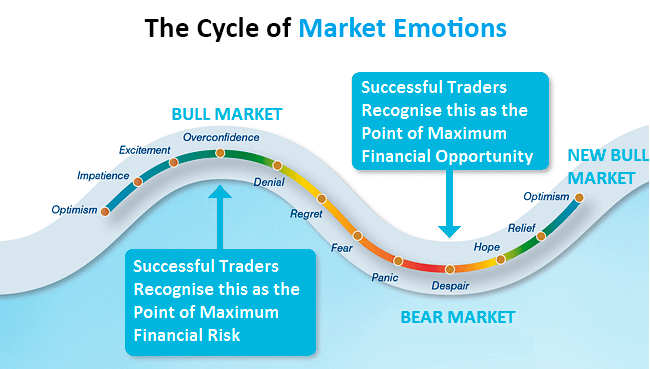
\includegraphics[width=0.7\textwidth]{img/trading-psychology.png}
\label{figure:trading-psychology}
\end{figure}

Stopping a trade does not only involve emotions, as a thorough analysis of the
market, about the current's account financial situation and the trades
themselves needs to be performed \cite{Kadiri2015}. Regarding about the first
step -- an analysis of the market -- it is worth mentioning that these analyses
are usually different than those performed when deciding when to start trading a
market \cite{Conrad1998} \cite{Muller1997}. For example, in a stagnated market
one could decide not to trade a market, but this does not necessarily mean that
one should close trade orders in this situation; one could consider that this is
a moment where trades need to be held until further price movements take
place. A trader can also decide to \textit{partially} stop a trade; that is, a
trader can decide to sell a certain amount of units from a trade, for
example. Likewise, a trader can decide to acquire more units from the asset.

It is usual that a trader \textit{diversifies} its trading portfolio
\cite{Muller1997}. Diversifying means that a trader starts trading a number of
financial markets instead of focusing on a single market. The advantages of this
are that the risk diminishes, as the profits of trading some markets can
compensate the losses obtained from trading other markets
\cite{Muller1997}. Diversification can then make trading strategies even more
complex, as a trader now needs to take into consideration different
markets. Additionally, markets usually affect the price movements of other
markets, for example, if wheat price goes up, this can directly impact the price
of McDonald's stock prices, as many of their products contain wheat-based
ingredients. Furthermore, if McDonald's stock market is severely affected, this
could negatively impact the United States' economy, as McDonald's is one of the
most profitable companies in this country. Depending on the robustness of a
trading strategy, all of these aspects can be considered to take a decision.

Trading strategies have existed since the activity of trading was created.  To
illustrate this, one can consider how the Japanese traded certain commodity
markets, such as the rice market, using strategies based on candlestick patterns
\cite{Nison1991}. The Japanese charted the prices by representing the open,
highest, lowest and close prices for a period of time using figures that
resemble candles and their wicks, as the those seen in Figure
\ref{figure:candlestick-chart}. The body of a candle in this type of charts
represents the opening and the closing prices of a session, while the wick
represents the lowest and highest prices that occured during the session.

%% These two will be redesigned to match the thesis document style
\begin{figure}
\caption{Example of a candlestick chart}
\centering

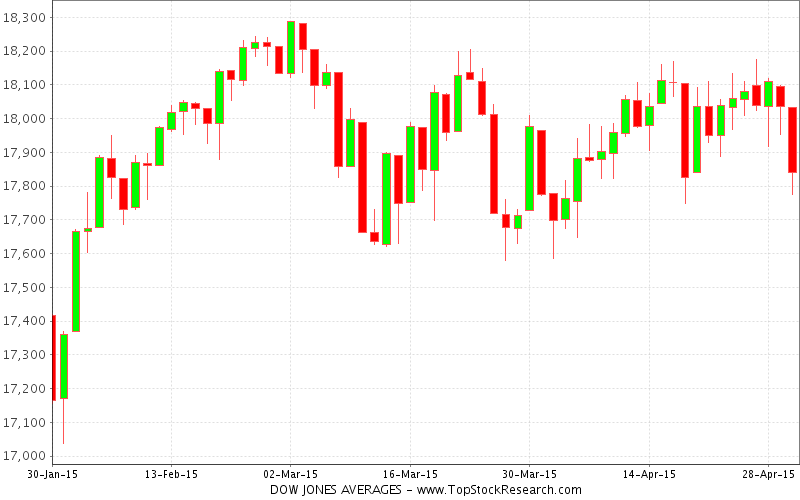
\includegraphics[width=0.7\textwidth]{img/candlestick-chart.png}
\label{figure:candlestick-chart}
\end{figure}

Japanese traders noticed patterns that emerged in the candlestick charts. These
patterns helped the traders to understand the current situation of a financial
market and to take decisions based on these assumptions. Some example patterns
are shown in Figure \ref{figure:candlestick-patterns}. For example, if a
``bullish engulfing'' or a ``rising sun'' candlestick pattern appears in the chart
of a market, this is considered as a sign of a following uptrend -- which means
that prices will increase. In contrast, if a ``bearish engulfing'' or ``dark cloud
cover'' candlestick pattern appears, this signs a following downtrend -- which
means that prices will decrease. Additionally, there are patterns that indicate
that a market will start stagnating, such as the ``harami'' candlestick
pattern. It is worth noting that these candlestick patterns are still used in
modern trading strategies \cite{Nison1991}.

All the processes described above can be performed manually, i.e. a trader can
look at price charts and start identifying candlestick patterns, draw moving
averages over the chart, decide on the number of units to buy or sell, decide on
take profit and stop loss levels, etc. However, with the introduction of
computers to the financial world in the mid 20th century, automated or
algorithmic trading was also introduced \cite{Hendershott2011}. Algorithmic
trading help traders to partially or totally delegate trading tasks to computer
software, where buy or sell transactions occur when a set of conditions are
met. In this thesis, an automated trading strategy is part of the proposed
method.

\begin{figure}
\caption{Example of candlestick patterns}
\centering
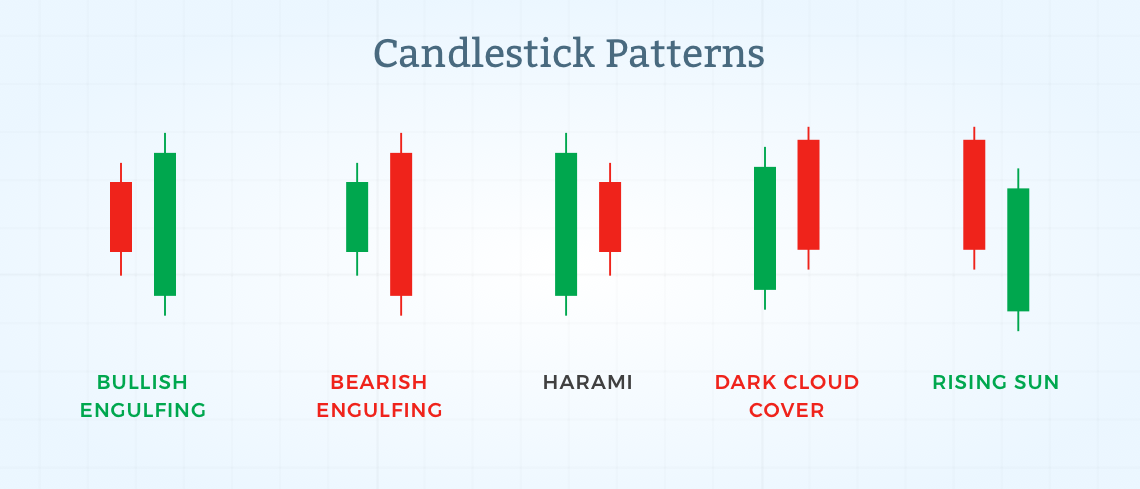
\includegraphics[width=0.7\textwidth]{img/candlestick-patterns.png}
\label{figure:candlestick-patterns}
\end{figure}

\section{Technical Analysis}
\label{section:technical-analysis}

Since many decades ago, financial traders have implemented statistical models to
forecast time-series, as part of a field called technical analysis
\cite{Lo2000}. This type of market analysis is characterized by using past
financial data to describe certain aspects of a market, such as its volatility,
trend, and momentum \cite{Achelis2000}. These indicators receive the name of
technical indicators. Some examples of technical indicators are those created by
Welles Wilder, such as the Relative Strength Index (RSI) and the Average
Directional Index \cite{Wilder1978}, and an example of an oscillator, which is a
type of technical indicator which usually tells if a market is overbought or
oversold, is the Stochastic Oscillator \cite{Schirding1984}, created by George
Lane. In contrast to technical analysis, fundamental analysis relies on the
examination of the underlying forces that affect a particular financial market
(or several of them), instead of just relying on the price movements in a
time-series. As an example of fundamental analysis, a trader can use the
financial statements of a public company to estimate if the price of their stock
will rise.

A more modern approach to perform these analyses is to use machine learning
techniques. Using machine learning algorithms, researchers create regression
models using technical or fundamental indicators as training datasets
\cite{Connor2005}.  Examples of regression techniques are autoregression
\cite{burg1968new}, symbolic regression \cite{billard2002symbolic}, and linear
regression \cite{kutner2004applied}. Other more elaborated techniques exist in
machine learning for regression or curve-fitting tasks, such as the use of
artificial neural networks \cite{melin2007hybrid} and support vector regression
\cite{basak2007support}.

\subsection{Retracements in Financial Markets}
\label{subsection:retracements-in-financial-markets}

A retracement in a financial market is any market price movement that goes
against a clear trend in a determined timeframe, but where the magnitude is not
significant enough to point to a reversal in the market's direction. For
example, if a stock market has been going upwards in price for the past three
months, and in the past week the price went downwards, this movement could be
considered a retracement. The retracement movement is confirmed once the market
retakes the general price direction. If the market never retakes this general
direction, a reversal is said to have occurred. An example of retracements in a
financial market price chart can be seen in Figure
\ref{figure:retracements-in-financial-market}.

\begin{figure}
\caption{Example of retracements in a financial market price chart} \centering
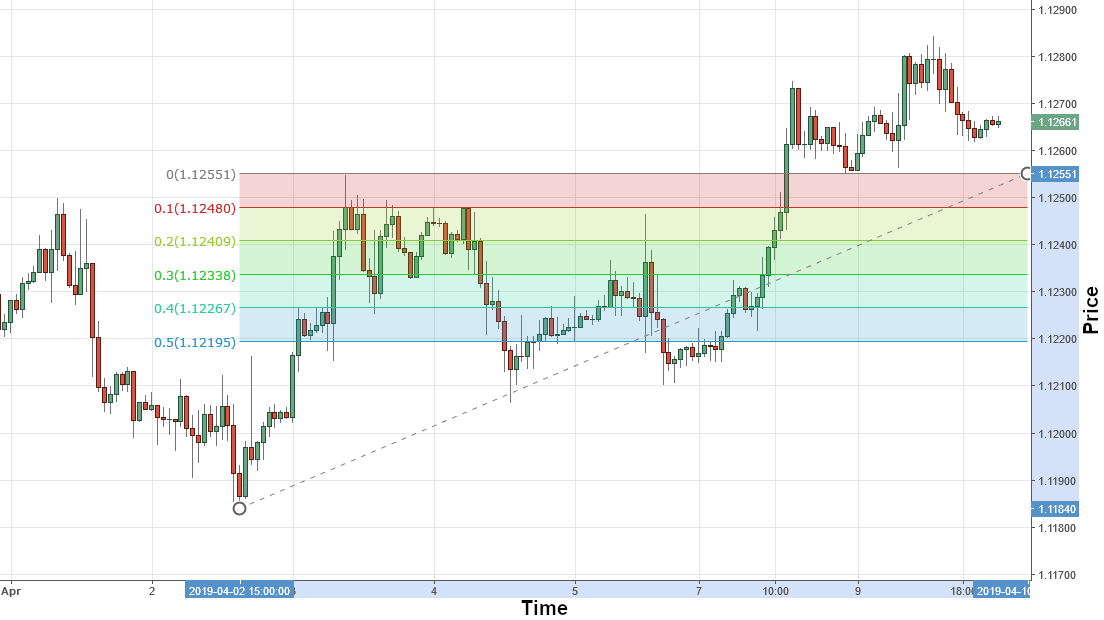
\includegraphics[width=0.7\textwidth]{img/retracements.png}
\label{figure:retracements-in-financial-market}
\end{figure}

A special type of retracements are Fibonacci retracements. In this type of
retracements, the market usually follow retracement movements that correspond to
Fibonacci ratios. For example, if a market has been following an uptrend in its
prices for the past 1000 units, and the market suffers a retracement of
approximately 382 units, it is said to be a Fibonacci retracement, as this
retracement follows a ratio of 0.382. Fibonacci retracements commonly occur
in financial market price charts. An example of fibonacci retracements can be
seen in Figure \ref{figure:fibonacci-retracements-in-financial-market}. It is
worth to mention that retracements do not always occur and they do not follow
the ratios exactly.

% Seems like ``retracements'' are heuristics. You should make this clear, we
% do not want the readers to think they are proven facts, or worst, that
% they think we are treating them as if they where. 

\begin{figure}
\caption{Example of Fibonacci retracements in a financial market price chart}
\centering
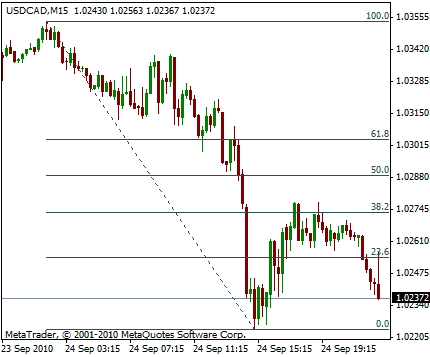
\includegraphics[width=0.7\textwidth]{img/fibonacci-retracements.png}
\label{figure:fibonacci-retracements-in-financial-market}
\end{figure}

\section{Computational Intelligence}
\label{section:computational-intelligence}

Computational intelligence is a field of computer science similar to artificial
intelligence. In contrast to artificial intelligence, where symbolic logic is
used to represent reasoning, computational intelligence relies on statistical
and bio-inspired approaches
\cite{JangJyh-ShingRogerandSunChuen-TsaiandMizutaniEijiandHo1998}. As the models
generated by computational intelligence are often not exact, but rather an
approximation to the problem it is modelling, it is sometimes also called soft
computing.

The following Sections discuss the computational intelligence techniques that
are used in the proposed method of this thesis.

\subsection{Fuzzy Sets}
\label{subsection:fuzzy-sets}

A traditional set is a collection of items that share a common
characteristic. This characteristic serves as a membership, because all the
items in a universe either have that characteristic -- and then the item is part
of the set -- or it does not have it -- and then the item is not part of the
set. Traditional sets can be extended to fuzzy sets, as explained by Zadeh
\cite{Zadeh1965}. Fuzzy sets are then a generalization of traditional sets,
i.e. any traditional set can be represented as a fuzzy set. The difference
between these two types of sets lies in the concept of membership: memberships
are not only used to represent binary outcomes, i.e. \textit{true} or
\textit{false}, but a possibly infinite number of outcomes. An item can now be
partially a member of a set, and the only way an item is not part of such set is
if its membership is totally \textit{false}. In order to represent this grade of
membership one can use real numbers. Thus, one can say, for example, that an
item is \textit{0.7 green}, \textit{0.5 blue} and \textit{0.0 red}. These values
can represent an adverb and an adjective, such as ``very green,'' ``somewhat blue''
and ``not red at all.'' This is especially useful when designing fuzzy systems
(see Subsection \ref{subsection:fuzzy-systems}).


\subsection{Fuzzy Systems}
\label{subsection:fuzzy-systems}

In traditional logic one can generate logical inferences, such as \textit{if
  it's raining, then there are clouds in the sky}. In a similar fashion, one can
use fuzzy sets to represent the antecedents and consequents in a logical
inference process. For example, one can extend the previous example to:
\textit{if it's raining a lot, then there are many clouds in the sky}.

There is a number of ways in which one can construct a fuzzy inference system,
where one or more inputs or antecedents can be used to generate one or more
outputs or consequents. Arguably, the two most popular types of fuzzy inference
systems are the ones created by Mamdani and Assilian \cite{Mamdani1975}, and
Takagi and Sugeno \cite{Takagi1985}. These systems use a series of fuzzy sets to
represent the relationship between an input and its grade of membership to a
set. These sets usually represent adjectives that describe the inputs, and are
also considered to be the antecedents in the fuzzy inference system. For
example, an input of 0.8 can represent a ``very high'' value. After obtaining
these grades of membership, one can use these values to ``fire'' or ``activate'' the
consequents. In the case of a Mamdani system, the consequents are represented as
fuzzy sets, just like the antecedents. In contrast, in a Sugeno system,
consequents are represented by mathematical functions. A set of rules is used to
determine the relationship between the antecedents and the consequents, for
example: \textit{if food quality is high then tip is high}. The aforementioned
rule is creating a relationship between the fuzzy set that represents ``high food
quality'' in the antecedents, and the fuzzy set that represents ``high tip'' in the
consequents. Further continuing with the example, if ``food quality'' is
represented by a value of 0.8, the rule that creates the relationship between
``food quality'' and ``tip'' could determine a ``tip'' of 0.8 too, depending on what
membership function and what parameters are decided to be used to represent
each.

It has been explained how a relationship between antecedents and consequents can
be constructed in a fuzzy inference system. Nevertheless, the most interesting
problem arises when a problem involves several fuzzy sets to represent different
adjectives for single antecedents or consequents. In these cases, depending on
the fuzzy rules, a number of consequents can be fired according to the inputs to
the system. As seen in Figure \ref{figure:antecedents}, the input -- represented
by the dotted vertical black line -- is associated with three fuzzy triangular
sets or antecedents, where it ``activates'' two of them. According to a set of
fuzzy rules, it then fires a set of triangular fuzzy sets that represent the
consequents, as seen in Figure \ref{figure:consequents}.

The fuzzy sets that represent the consequents are cut, and new shapes are
obtained using those cuts, as represented by the green shapes in Figure
\ref{figure:consequents}. These shapes are aggregated and result in the output
of the fuzzy inference system, and this result can then be defuzzified
(converted from a fuzzy set to a scalar or crisp value) using different methods,
such as obtaining the centroid of the shape. In this example, a Mamdani fuzzy
inference system is considered; in the case of a Sugeno system, for example, the
antecedents would be represented by arbitrary mathematical functions, instead of
membership functions representing shapes such as the triangles in the example
presented above.

\begin{figure}
\caption{Antecedents}
\centering
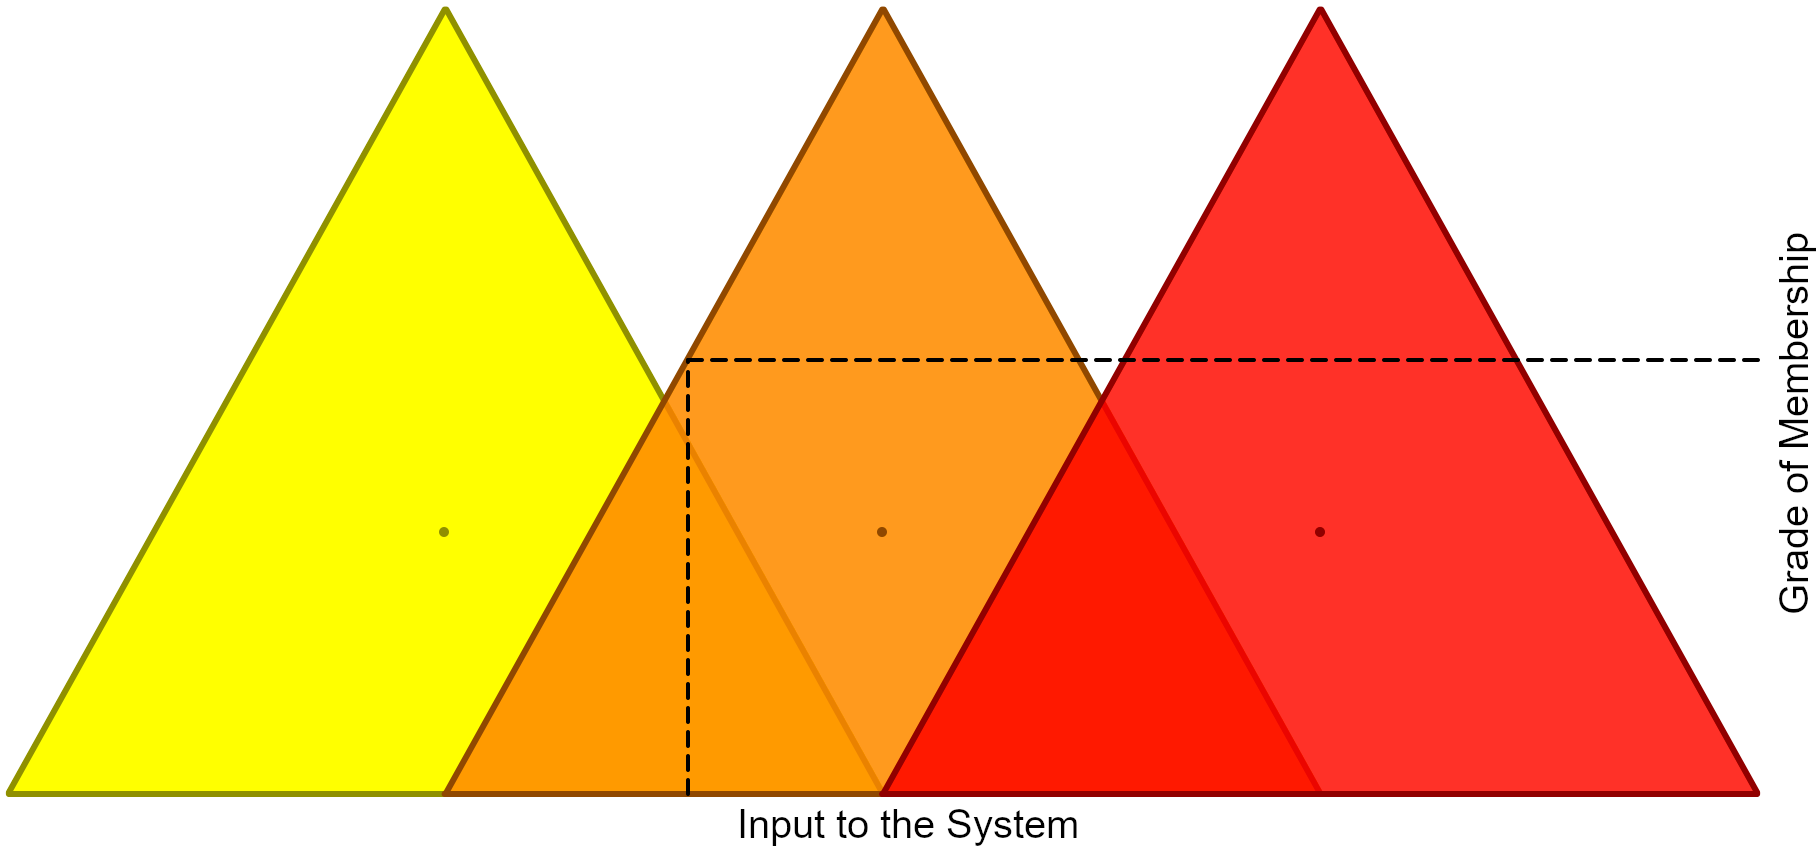
\includegraphics[width=0.7\textwidth]{img/antecedents.png}
\label{figure:antecedents}
\end{figure}

\begin{figure}
\caption{Consequents}
\centering
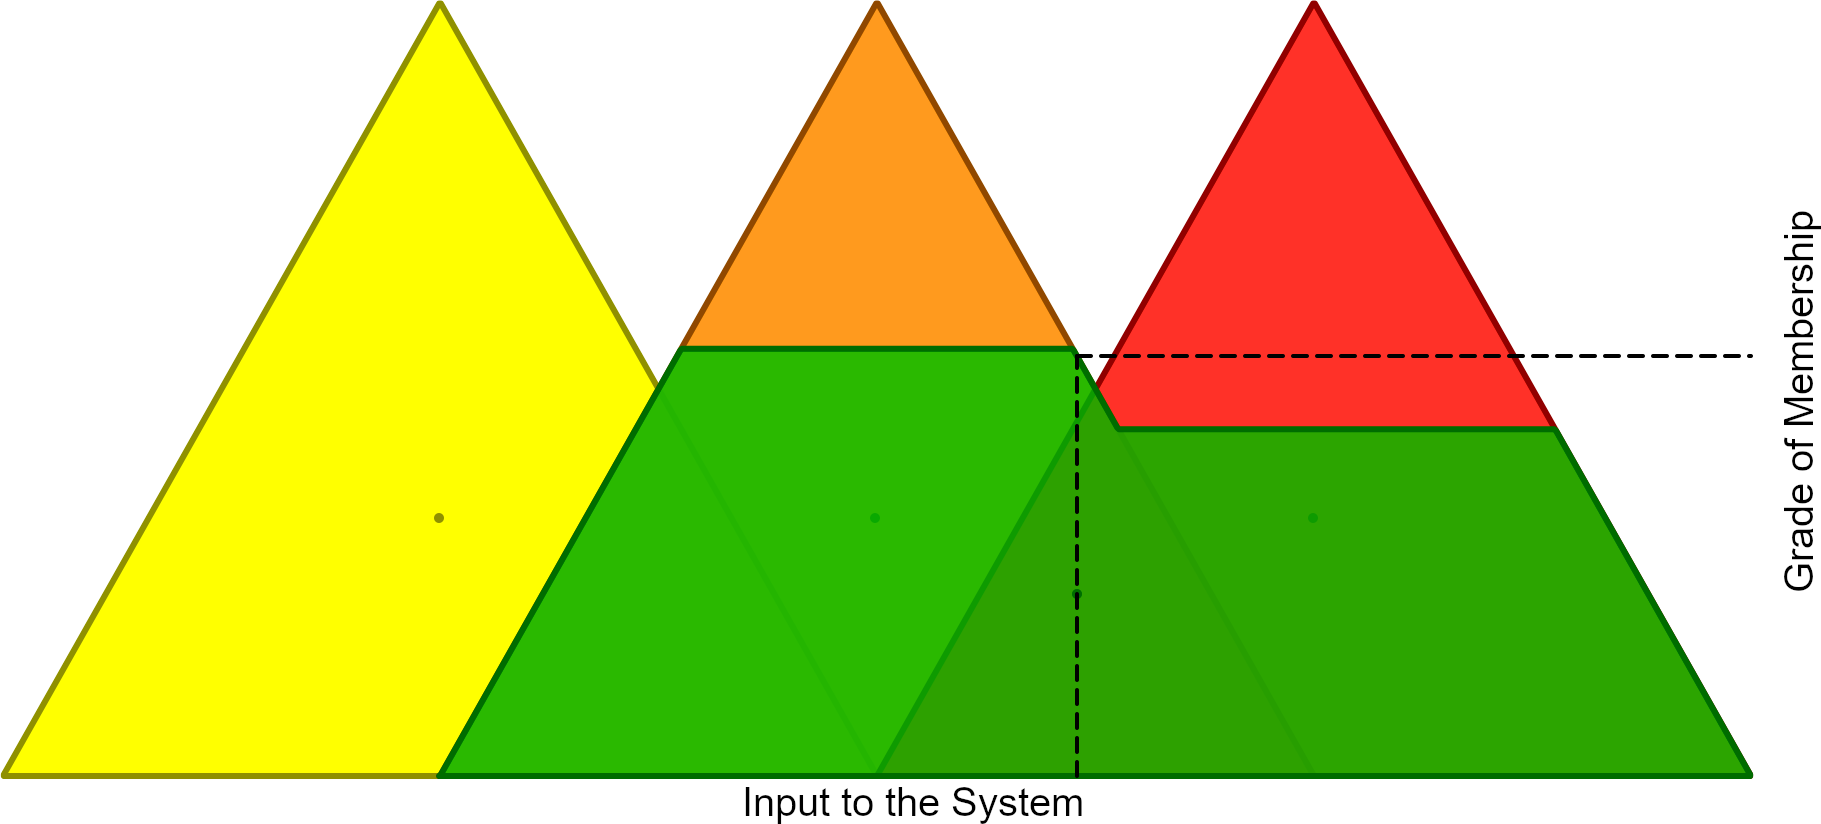
\includegraphics[width=0.7\textwidth]{img/consequents.png}
\label{figure:consequents}
\end{figure}

\subsection{Fuzzy Systems Software}
\label{subsection:fuzzy-systems-software}

There are a number of implementations of fuzzy systems toolboxes or libraries
where a programmer can design a fuzzy system to be integrated with other
software projects or used as stand-alone applications. The vast majority of this
software is dedicated to the creation of type-1 fuzzy systems, i.e. systems that
do not consider uncertainty in the grade of membership of their antecedents or
consequents.

Wagner presents a robust implementation of FISs developed in Java in
\cite{Wagner2013}. Although the toolkit does not provide many tools
for representing a FIS graphically or for interacting with one, the
implementation provides libraries for building type-1, interval type-2, and
generalized type-2 fuzzy systems.

Moreover, the work by Castro et al. \cite{castro2007interval} provides the same
capabilities as the work by Wagner, but in this case it is an implementation in
Matlab. A direct disadvantage of using this programming language is that Matlab
is not a free nor open source software.  Nevertheless, the language is still
widely used in the scientific community. Furthermore, this implementation
follows an interface similar to the one provided by Matlab's fuzzy logic
toolbox, and provides more robust graphical implementations than the current
version of Wagner's toolkit.

\subsection{Intuitionistic Fuzzy Sets}
\label{subsection:intuitionistic-fuzzy-sets}

In contrast to the traditional fuzzy sets discussed in Subsection
\ref{subsection:fuzzy-sets}, intuitionistic fuzzy sets consider a grade of
non-membership in addition to a grade of membership associated to an element in
the fuzzy set, as expressed by \ref{eq:ifs-definition}. Intuitionistic fuzzy
sets were defined by Atanassov in \cite{Atanassov1986}.

% intuitionistic fuzzy set
\begin{equation}
  \label{eq:ifs-definition}
  A^{*} = \{\langle x, \mu _{A} (x), \nu _{A} (x) \rangle | x \in E\}
\end{equation}

For every of the elements contained in an intuitionistic fuzzy set,
\ref{eq:intuitionistic-interval} must hold true.

% intuitionistic interval
\begin{equation}
  \label{eq:intuitionistic-interval}
  0 \leq \mu_{A}(x) + \nu_{A}(x) \leq 1
\end{equation}

Intuitionistic fuzzy sets are an extension to traditional fuzzy sets, as any
traditional fuzzy set can be expressed as a particular case of an intuitionistic
fuzzy set, as in \ref{eq:ifs-form}.

% every ordinary fuzzy set has the form
\begin{equation}
  \label{eq:ifs-form}
  \{ \langle x, \mu_{A}(x), 1 - \mu_{A}(x) \rangle | x \in E \}
\end{equation}

If the sum of the membership $\mu_{A}(x)$ and non-membership $\nu_{A}(x)$ of an
element is less than $1$, the concept of indeterminacy or hesitancy arises,
which is described by \ref{eq:indeterminacy}. Indeterminacy is used to represent
doubt in the grade of membership of an element in an intuitionistic fuzzy set
and is described by \ref{eq:indeterminacy}.

% if
\begin{equation}
  \label{eq:indeterminacy}
  \pi_{A}(x) = 1 - \mu_{A}(x) - \nu_{A}(x)
\end{equation}

Traditional fuzzy sets can be extended to increase their capabilities of
representing uncertainty by introducing the concept of footprint of
uncertainty. A footprint of uncertainty is achieved by extending the membership
function, where each of its values are now fuzzy sets themselves, instead of
crisp values. This type of traditional fuzzy sets are commonly labeled as type-2
fuzzy sets in the literature \cite{Mendel2006}.

Indeterminacy serves a different purpose than the one of footprint of
uncertainty. Instead of extending the uncertainty provided by traditional fuzzy
sets, indeterminacy helps to model doubt \cite{Xu2007}. For example, if
traditional fuzzy sets can model the following sentence: ``the object is very
hot'', indeterminacy can model ``it is unsure that the object is very hot''.

\subsection{Intuitionistic Fuzzy Systems}
\label{subsection:intuitionistic-fuzzy-systems}

Human beings tend to express their knowledge using natural language and certain
words to describe abstract objects or experiences in fuzzy terms. For example,
after generating a financial report, one is interested in knowing if an
organization is ``doing well,'' or if it is ``not profitable enough.'' The
previous examples are fuzzy statements that need to be inferred from data, but
this data can also be uncertain (e.g. noise is present in the data). For that
reason, fuzzy sets have been proposed for data modeling and knowledge
representation. On the other hand, fuzzy inference systems (FIS) have been
applied in the construction of control and pattern recognition systems also
based on such fuzzy data. Nevertheless, occasionally there are situations where
a traditional FIS can not properly model certain data sets, due to high levels
of uncertainty present in the data (e.g., noise). As a consequence, researchers
have extended fuzzy sets and fuzzy logic theory to allow the construction of
systems that can successfully represent noisy data.

One of the extensions to fuzzy sets are type-2 fuzzy sets \cite{Mendel2002}. The
idea behind this extension is to add uncertainty to the membership of an element
to a fuzzy set. In other words, an element will have a grade of membership to a
fuzzy set, and this grade of membership will be represented as another fuzzy
set. For example, this technique allows a fuzzy system to be more resilient to
data with many outliers; it will be easier for a type-2 fuzzy system to create a
generalized model of the data than a type-1 fuzzy system. Many works have
incorporated type-2 fuzzy sets into their systems and have obtained better
performance when compared to their traditional or type-1 fuzzy sets counterparts
\cite{Liang2000}. Despite this increase in capabilities for handling
uncertainty, type-2 fuzzy systems have the disadvantage of being significantly
slower than type-1 systems \cite{Sepulveda2012}. The reason for this penalty in
performance is mainly due to how a type-2 fuzzy system is implemented, that is,
the programming language used for it and what type of programming techniques
were used to implement the fuzzy theory. One way to mitigate this problem is to
restrict the fuzzy sets that represent the grade of membership for an element,
in order to simplify the calculations needed for the system to generate
inferences, and therefore quicken the process. Interval type-2 fuzzy systems
were the result of implementing this idea, which are a particular case of
general type-2 fuzzy systems \cite{Mendel2006}. Another way is to reduce the
complexity of the algorithm, such as in the case of the work from Karnik and
Mendel \cite{Karnik2001}.

Fuzzy sets can also be extended to intuitionistic fuzzy sets (IFS), which are
proposed by Atanassov in \cite{Atanassov1986}. As in the case of type-2 fuzzy
sets, IFS increase the capabilities of a traditional fuzzy set to represent
uncertainty, by introducing the concept of indeterminacy. Basically an element
that belongs to an IFS is described by a grade of membership (\(\mu\)) and a
grade of non-membership (\(\nu\)). One can express how well an element belongs
to a fuzzy set and how well an element does not belong to that fuzzy set as
well. As a consequence, the sum of the values for the membership and
non-membership are not always equal to 1, and \(1-(\mu + \nu)\) will be known as
indeterminacy, which is represented by the symbol \(\pi\). FISs that implement
intuitionistic fuzzy sets have at least two advantages: 1) they can handle more
uncertainty than traditional FISs and can process their inferences to crisp
values with almost no resource performance impact, and 2) they can still be
extended to use type-2 fuzzy sets, giving as a result an intuitionistic type-2
FIS.

The use of IFSs in a traditional FIS should enable the handling of more
uncertainty, and one could prefer an intuitionistic FIS (IFIS) to obtain better
accuracies without sacrificing time performance, as inferences in a type-2 FIS
(T2-FIS) are very time consuming compared to a type-1 FIS (T1-FIS). This is a
consequence of the complex type reducing procedure that is involved in the
defuzzification stage in a T2-FIS \cite{Liang2000}. Several improvements to the
algorithms involved in the inference process in a T2-FIS have been proposed to
alleviate this problem, such as the Karnik-Mendel algorithm \cite{Karnik2001}
and shadowed sets \cite{Pedrycz1998}. Nevertheless, a T2-FIS is usually several
times slower than a T1-FIS. Because of this time performance impact, many works
that require handling more uncertainty than a T1-FIS use a particular case of
T2-FIS, the interval T2-FIS (IT2-FIS) \cite{Liang2000}, which is faster than a
general T2-FIS (GT2-FIS). A type-1 IFIS (T1-IFIS) should perform better than a
T1-FIS in terms of accuracy (in problems involving data with high levels of
uncertainty), and should be faster than a T2-FIS. Furthermore, IFSs can be
implemented as part of a T2-FIS, giving as a result a type-2 IFIS.

\subsection{Membership and Non-Membership Functions Design}
\label{subsection:membership-and-non-membership-functions-design}

At the time of writing this thesis, there are not many works involving Mamdani
type intuitionistic inference systems yet, and the author of this work is only
aware of the work by O. Castillo et al. \cite{castillo2007intuitionistic}, and
A. Hernandez-Aguila and M. Garcia-Valdez \cite{Hernandez-aguila2016}. As a
consequence of this lack of works involving Mamdani FISs, there is not a common
way to graphically represent an IFS for its use as membership and non-membership
functions for an IFIS. Additionally, there is not a common way to graphically
represent the architecture of an IFIS.

In this thesis we use the method to graphically represent IFISs' architectures
proposed in \cite{Hernandez-aguila2017-2} in which the author of this thesis
participated. Figure \ref{figure:ifs-proposed} depicts an example of an IFS that
uses the graphical representation proposed in the aforementioned work, and
Figure \ref{figure:ifs-proposed-diff-mu-sd} shows a similar IFS where the mean
of the non-membership function is different than the mean of the membership
function. Also, it is noteworthy how the membership function has core in 0.7 --
instead of 1, as in traditional fuzzy sets -- and the non-membership function
has a core in 0.3.

\begin{figure}
\caption{Example of an intuitionistic fuzzy set with the proposed graphical
  representation} \centering 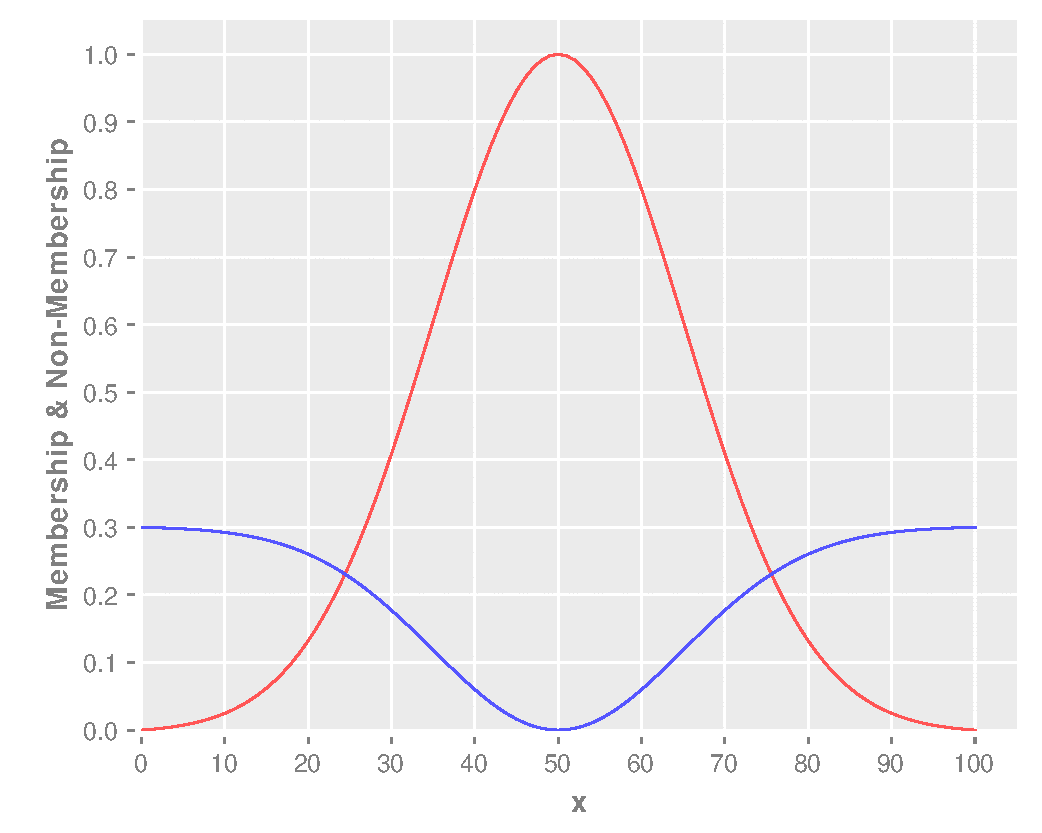
\includegraphics[width=0.7\textwidth]{img/ifs.pdf}
\label{figure:ifs-proposed}
\end{figure}

\begin{figure}
\caption{Example of an intuitionistic fuzzy set with the proposed graphical
  representation with different mean and indeterminacy} \centering
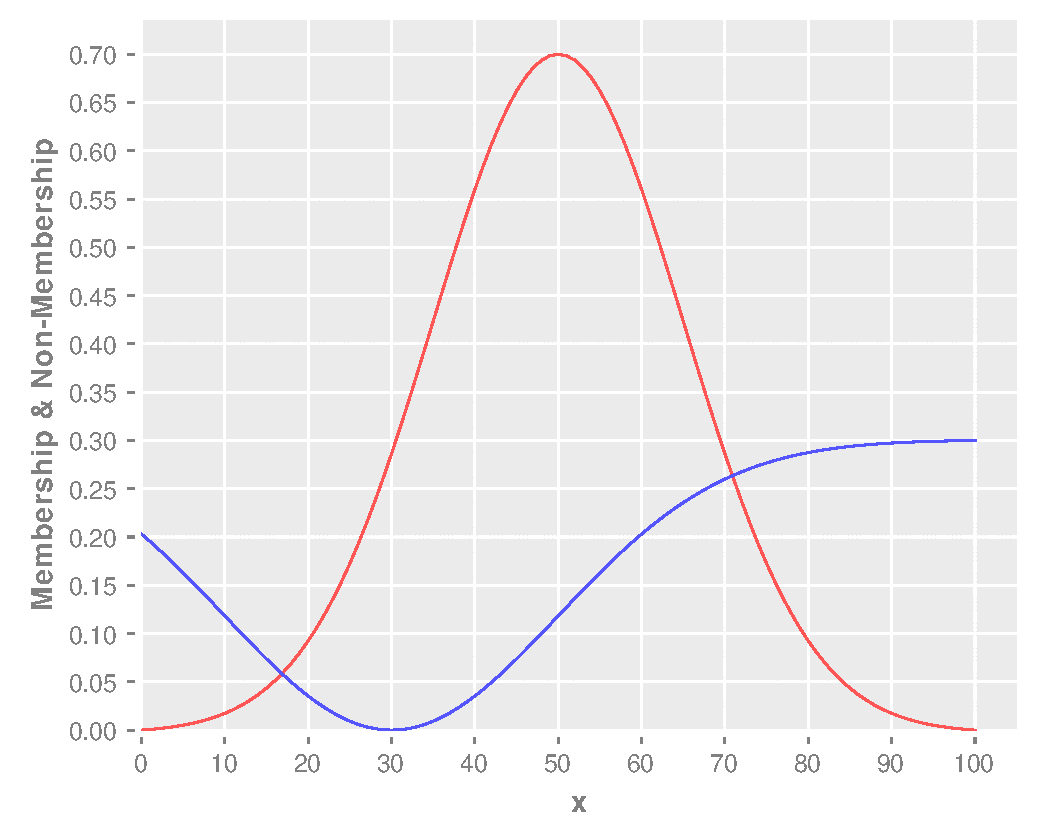
\includegraphics[width=0.7\textwidth]{img/ifs-diff-mu-sd.pdf}
\label{figure:ifs-proposed-diff-mu-sd}
\end{figure}

\section{Genetic Algorithms}
\label{section:genetic-algorithms}

A genetic algorithm (GA) is an optimization algorithm inspired in evolution. For
this reason GAs are considered to be part of a subfield of optimization
algorithms called evolutionary algorithms \cite{Whitley1994}. A GA proposes an
initial set of possible solutions to a problem -- usually called a
population. Each solution in this population is called a chromosome and
sometimes they are referred as individuals. The population is evaluated against
a fitness function, which is going to determine each of the individuals'
performance when trying to solve a particular problem. This problem commonly
involves finding sets of parameters that will cause a system to minimize or
maximize an error.

The population in a GA undergoes an evolutionary process that involves the
crossover among the fittest individuals in the population, and the elimination
of those individuals that perform the worst according to the fitness
function. The crossover process is usually performed by recombining the genes in
the chromosomes of the selected individuals -- which are usually the
fittest. The aforementioned process is usually repeated for a number of
iterations, which are commonly called generations.

In GAs and other evolutionary algorithms, the population will usually start to
become more fit to solve a problem after a series of generations, but it is
common that none of the individuals finds the best possible solution for the
problem. Furthermore, running an evolutionary algorithm several times will most
likely yield different results, as the initial population of solutions are
randomly generated. For this reason, evolutionary algorithms are said to be
meta-heuristic search algorithms, as they find suboptimal solutions to other
problems that do not directly involve the evolutionary algorithm, and they are
also considered stochastic algorithms \cite{Harik1999}.

\section{Multi-agent Systems and Models}
\label{section:multi-agent-systems-and-models}

A multi-agent system is software that solves a problem using agents. Agents can
be seen themselves as programs that interact with their environment, which may
include other agents. Agents in the proposed method in this paper follow the
structure suggested by Shoham in \cite{Shoham1993}, where agents have beliefs
and rules. Beliefs are used by agents to arrive to an interpretation of their
environment, and rules are used to arrive to actions to be performed by the
agent towards their environment. The agents in the system are constantly sensing
their environment to determine what actions to take according to their beliefs
and rules. Multi-agent systems have the objective of solving a practical
problem, unlike agent-based models which are more focused to providing a
simulation of a problem.

As mentioned before, agents can also be used to create agent-based models. These
models are used to represent a problem so a human being can analyze it and infer
new knowledge from it, or it can be used to better understand a problem.

The proposed method in this paper is both a multi-agent system and an
agent-based model. It is a multi-agent system in the sense that it can be used
to create a trading strategy, and it is an agent-based model because the agents
in the system can be analyzed to understand the state of the market that is
serving as the system's environment.
